\documentclass{article}%
\usepackage[T1]{fontenc}%
\usepackage[utf8]{inputenc}%
\usepackage{lmodern}%
\usepackage{textcomp}%
\usepackage{lastpage}%
\usepackage[head=40pt,margin=0.5in,bottom=0.6in]{geometry}%
\usepackage{graphicx}%
%
\title{\textbf{Siga en vivo audiencia del Senado sobre las relaciones de EE UU y Venezuela}}%
\author{EL NACIONAL}%
\date{07/03/2019}%
%
\begin{document}%
\normalsize%
\maketitle%
\textbf{URL: }%
http://www.el{-}nacional.com/noticias/siga{-}vivo{-}audiencia{-}del{-}senado{-}sobre{-}las{-}relaciones{-}venezuela\_273737\newline%
%
\textbf{Periodico: }%
EN, %
ID: %
273737, %
Seccion: %
EE UU\newline%
%
\textbf{Palabras Claves: }%
Nicolás Maduro, Estados Unidos, Marco Rubio, Crisis humanitaria\newline%
%
\textbf{Derecho: }%
2.1%
, Otros Derechos: %
\newline%
%
\textbf{\textit{En la reunión se discutirá sobre la crisis en el país y el camino hacia una transición democrática}}%
\newline%
\newline%
%
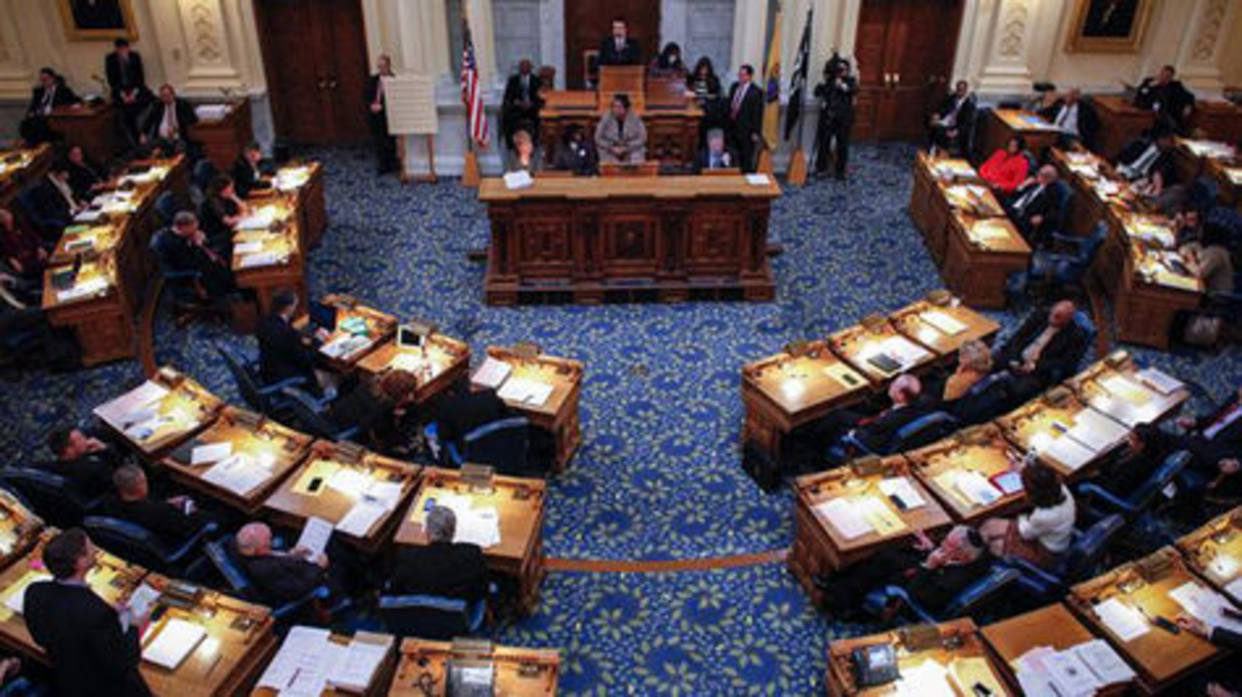
\includegraphics[width=300px]{EN_273737.jpg}%
\newline%
%
Este jueves se lleva a cabo una audiencia del Senado sobre las relaciones entre EE UU y Venezuela y el camino hacia una transición democrática.%
\newline%
%
El senador republicano, Marco Rubio, resaltó durante su intervención que la~crisis en Venezuela no es producto de las sanciones, sino del robo del gobierno y sus secuaces.%
\newline%
%
En el encuentro también se esperan declaraciones de~Elliott~Abrams, encargado especial de EE UU para la crisis en Venezuela.%
\newline%
%
Para escuchar la transmisión en vivo y seguir minuto a minuto la información visite:~VOA%
\newline%
%
\end{document}